% !TEX program = xelatex
% Отчёт о лабораторной работе № 2 «Синтез комбинационных суммирующих устройств. АЛУ»
% Компиляция: xelatex report.tex (дважды — для содержания и ссылок)
% Рядом с файлом должны лежать рисунки lab2_*.png
\documentclass[14pt,a4paper]{extarticle}

% ---------- Шрифты и язык ----------
\usepackage{fontspec}
\IfFontExistsTF{Times New Roman}
  {\setmainfont{Times New Roman}}
  {\setmainfont{Liberation Serif}}
\IfFontExistsTF{Courier New}
  {\setmonofont{Courier New}}
  {\setmonofont{Liberation Mono}}
% Язык: babel (совместим со старыми и новыми версиями L3; polyglossia v2.8 требует свежего l3kernel)
\usepackage[english]{babel}
\babelprovide[import, main]{russian}
\usepackage{unicode-math}
\setmathfont{latinmodern-math.otf}
\IfFontExistsTF{Times New Roman}
  {\setmathfont[range={up/{latin,Latin,num}}]{Times New Roman}
   \setmathfont[range={it/{latin,Latin}}]{Times New Roman Italic}}
  {\setmathfont[range={up/{latin,Latin,num}}]{Liberation Serif}
   \setmathfont[range={it/{latin,Latin}}]{Liberation Serif Italic}}

% ---------- Поля и интервалы (ГОСТ 7.32-2001, п. 6.1.1) ----------
\usepackage[left=30mm,right=10mm,top=15mm,bottom=20mm,footskip=10mm]{geometry}
\usepackage{setspace}
\onehalfspacing
\setlength{\parindent}{1.25cm}
\usepackage{indentfirst}
\setlength{\parskip}{0pt}
\sloppy

% ---------- Заголовки ----------
\usepackage{titlesec}
\titleformat{\section}{\normalfont\bfseries}{\thesection}{0.6em}{}
\titleformat{\subsection}{\normalfont\bfseries}{\thesubsection}{0.6em}{}
\titlespacing*{\section}{\parindent}{18pt}{12pt}
\titlespacing*{\subsection}{\parindent}{12pt}{6pt}
\renewcommand{\thesection}{\arabic{section}}
\renewcommand{\thesubsection}{\thesection.\arabic{subsection}}

% Структурные элементы без номера: с новой страницы, по центру, прописными
\newcommand{\structsection}[1]{%
  \clearpage
  \phantomsection
  \addcontentsline{toc}{section}{#1}%
  \begin{center}\textbf{#1}\end{center}\vspace{6pt}}

% ---------- Содержание (без tocloft — совместимо со старым ядром LaTeX) ----------
\makeatletter
\renewcommand{\tableofcontents}{%
  {\centering\textbf{СОДЕРЖАНИЕ}\par}\vspace{12pt}%
  \@starttoc{toc}}
\renewcommand*{\l@section}{\@dottedtocline{1}{0pt}{1.5em}}
\renewcommand*{\l@subsection}{\@dottedtocline{2}{1.5em}{2.3em}}
\renewcommand{\@pnumwidth}{1.8em}
\makeatother

% ---------- Подписи рисунков и таблиц (ГОСТ 7.32-2001, пп. 6.5, 6.6) ----------
\usepackage{caption}
\DeclareCaptionLabelSeparator{gost}{~---~}
\captionsetup{labelsep=gost, font={normalsize}, skip=6pt}
\captionsetup[figure]{name=Рисунок, justification=centering}
\captionsetup[table]{name=Таблица, justification=raggedright, singlelinecheck=false, position=top}

% ---------- Таблицы, графика, формулы ----------
\usepackage{graphicx}
\usepackage{float}
\usepackage{array,tabularx,makecell,multirow}
\renewcommand{\arraystretch}{1.15}
\newcolumntype{C}{>{\centering\arraybackslash}X}
\newcolumntype{L}{>{\raggedright\arraybackslash}X}
\usepackage{amsmath}
\usepackage{tikz}
\usetikzlibrary{arrows.meta,positioning,calc}
\usepackage{enumitem}
\setlist{nosep, leftmargin=*, labelindent=\parindent, itemindent=0pt}
\newlist{gostlist}{enumerate}{1}
% Буквенная нумерация перечислений по ГОСТ 2.105-95 (без букв ё, з, й, о, ч, ъ, ы, ь)
\newcommand{\gostletter}[1]{\ifcase#1\or а\or б\or в\or г\or д\or е\or ж\or и\or к\or л\or м\or н\or п\fi}
\newcommand{\gostlettercnt}[1]{\gostletter{\value{#1}}}
\AddEnumerateCounter{\gostlettercnt}{\gostletter}{м}
\setlist[gostlist]{label=\gostlettercnt*), leftmargin=*, labelindent=\parindent, nosep}
\newlist{dashlist}{itemize}{1}
\setlist[dashlist]{label=--, leftmargin=*, labelindent=\parindent, nosep}

\usepackage{listings}
\lstset{basicstyle=\ttfamily\small, columns=fullflexible, frame=single}

\usepackage[hidelinks]{hyperref}

% ---------- Колонтитулы: номер страницы внизу по центру ----------
\pagestyle{plain}

% ---------- Данные для титульного листа (заполнить) ----------
\newcommand{\StudentName}{Р.\,Ю.~Дужнов}
\newcommand{\StudentGroup}{5130201/50302}
\newcommand{\ReportDate}{24.09.2026}

% Обозначение инверсии
\newcommand{\inv}[1]{\overline{#1}}

\begin{document}
% ======================= ТИТУЛЬНЫЙ ЛИСТ =======================
\begin{titlepage}
\begin{singlespace}
\begin{center}
Министерство науки и высшего образования Российской Федерации\\[2pt]
Санкт-Петербургский политехнический университет Петра Великого\\[2pt]
Институт компьютерных наук и кибербезопасности\\[2pt]
Высшая школа технологий искусственного интеллекта

\vspace{5cm}

\textbf{ОТЧЁТ}\\[6pt]
\textbf{о лабораторной работе № 2}\\[12pt]
\textbf{«Синтез комбинационных суммирующих устройств. АЛУ»}\\[12pt]
по дисциплине «Основы архитектуры ЦВМ»
\end{center}

\vspace{4cm}

\noindent
\begin{tabular}{@{}p{7.2cm}p{3.6cm}l@{}}
Выполнил\\
студент гр. \StudentGroup & \underline{\hspace{3cm}} & \StudentName\\[22pt]
Проверил\\
доцент, к.\,т.\,н. & \underline{\hspace{3cm}} & Н.\,М.~Вербова\\
\end{tabular}

\vspace{1.2cm}
\noindent\hfill «\underline{\hspace{0.9cm}}» \underline{\hspace{3.2cm}} 2026 г.

\vfill
\begin{center}
Санкт-Петербург\\
2026
\end{center}
\end{singlespace}
\end{titlepage}
\setcounter{page}{2}

% ======================= СОДЕРЖАНИЕ =======================
\begin{singlespace}
\tableofcontents
\end{singlespace}

% ======================= ВВЕДЕНИЕ =======================
\structsection{ВВЕДЕНИЕ}

Объектом исследования являются комбинационные суммирующие устройства~--- полусумматор и одноразрядный сумматор~--- и четырёхразрядное арифметико-логическое устройство (АЛУ). Работа выполнена в соответствии с методическими указаниями~[1].

Цель работы~--- изучение принципов работы суммирующих устройств.

Для достижения цели решены следующие задачи:
\begin{gostlist}
\item синтезирована по заданной таблице истинности схема полусумматора, проверено её функционирование методом моделирования;
\item синтезирована по заданной таблице истинности схема одноразрядного комбинационного сумматора, проверено её функционирование методом моделирования;
\item изучен принцип работы четырёхразрядного АЛУ К155ИП3 (зарубежный аналог SN74181);
\item собрана схема исследования АЛУ К155ИП3 и исследована его работа в режимах логических и арифметических операций на заданных операндах.
\end{gostlist}

Моделирование выполнено в среде NI Multisim, являющейся развитием пакета Electronics Workbench, для которого составлены методические указания~[1].

% ======================= 1 =======================
\clearpage
\section{Теоретические сведения}

\subsection{Двоичное сложение}

Двоичное $n$-разрядное число представляется суммой степеней основания системы счисления с весами разрядов:
\begin{equation}
A = \sum_{i=0}^{n-1} a_i \cdot 2^i,
\end{equation}
\noindent где $A$~--- значение числа;\\
$a_i$~--- значение $i$-го разряда, $a_i \in \{0, 1\}$;\\
$n$~--- разрядность числа.

Сложение двоичных чисел выполняется поразрядно, начиная с младшего разряда, по тем же правилам, что и в десятичной системе счисления~[1]. В каждом разряде складываются два разряда операндов и перенос из младшего разряда; формируются разряд суммы и перенос в старший разряд.

\subsection{Полусумматор и сумматор}

Полусумматором называется комбинационная схема с двумя входами $X$, $Y$ и двумя выходами $S$ (сумма) и $P$ (перенос), выполняющая сложение двух одноразрядных двоичных чисел без учёта переноса из младшего разряда. Выход суммы полусумматора реализует функцию неравнозначности (суммы по модулю два)~[1].

Одноразрядным комбинационным (полным) сумматором называется комбинационная схема с тремя входами~--- разрядами операндов $X$, $Y$ и переносом из младшего разряда $Z$~--- и двумя выходами: суммой $S$ и переносом в старший разряд $P$~[1]. Многоразрядный сумматор строится цепочкой одноразрядных сумматоров, в которой выход переноса каждого разряда соединён со входом переноса следующего.

\subsection{Арифметико-логическое устройство}

Арифметико-логическим устройством называется комбинационный узел, выполняющий над двумя многоразрядными операндами набор арифметических и поразрядных логических операций, выбираемый управляющим кодом~[1]. Логические операции выполняются независимо в каждом разряде, арифметические~--- с распространением переноса между разрядами.

% ======================= 2 =======================
\section{Синтез полусумматора}

\subsection{Исходные данные}

Функционирование полусумматора задано таблицей истинности (таблица~\ref{tab:ha}).

\begin{table}[H]
\caption{Таблица истинности полусумматора}
\label{tab:ha}
\centering\small
\begin{tabularx}{0.7\textwidth}{|C|C|C|C|}
\hline
$X$ & $Y$ & $S$ & $P$ \\ \hline
0 & 0 & 0 & 0 \\ \hline
0 & 1 & 1 & 0 \\ \hline
1 & 0 & 1 & 0 \\ \hline
1 & 1 & 0 & 1 \\ \hline
\end{tabularx}
\end{table}

\subsection{Аналитические выражения}

По таблице~\ref{tab:ha} функция $S$ равна единице на наборах 01 и 10, функция $P$~--- на наборе 11. Запись функций в СДНФ даёт:
\begin{equation}
S = \inv{X} \cdot Y \vee X \cdot \inv{Y} = X \oplus Y,
\end{equation}
\begin{equation}
P = X \cdot Y,
\end{equation}
\noindent где $S$~--- разряд суммы;\\
$P$~--- перенос в старший разряд;\\
$X$, $Y$~--- слагаемые разряды;\\
$\oplus$~--- операция суммы по модулю два.

Конституенты $\inv{X} Y$ и $X \inv{Y}$ различаются значениями двух переменных, поэтому склеивание к выражению~(2) неприменимо; выражения~(2) и~(3) минимальны в базисе И, ИЛИ, НЕ.

\subsection{Варианты реализации}

Рассмотрены две модификации схемы полусумматора.

Модификация 1 реализует выражение~(2) непосредственно элементом «Исключающее ИЛИ», а выражение~(3)~--- элементом И (рисунок~\ref{fig:ha}, а). Модификация выбрана для моделирования, так как содержит минимальное число элементов.

Модификация 2 построена в базисе И, ИЛИ, НЕ. Для сокращения числа элементов выражение~(2) преобразовано так, чтобы использовать уже формируемый сигнал $X Y$:
\begin{equation}
S = \inv{X}\,Y \vee X\,\inv{Y} = (X \vee Y) \cdot (\inv{X} \vee \inv{Y}) = (X \vee Y) \cdot \inv{X \cdot Y},
\end{equation}
\noindent где $X$, $Y$~--- слагаемые разряды;\\
$S$~--- разряд суммы.

Второе равенство в~(4) получено раскрытием скобок с учётом $X \inv{X} = 0$ и $Y \inv{Y} = 0$, третье~--- по закону де Моргана. Схема модификации 2 приведена на рисунке~\ref{fig:ha}, б. Сложность вариантов по Квайну (суммарное число входов элементов) составляет 4 для модификации 1 (XOR2 и AND2) и 7 для модификации 2 (AND2, OR2, NOT, AND2).

\begin{figure}[H]
\centering
\begin{tikzpicture}[line width=0.5pt, font=\small, scale=1.2, every node/.style={transform shape}]
% ---- а) ----
\begin{scope}
\node[left] at (0,0.3) {$X$}; \node[left] at (0,-1.3) {$Y$};
\draw (0,0.3) -- (1.8,0.3); \draw (0,-1.3) -- (1.8,-1.3);
\fill (1.0,0.3) circle (1.6pt); \fill (1.4,-1.3) circle (1.6pt);
\draw (1.8,-0.1) rectangle (2.8,0.9); \node at (2.3,0.65) {=1};
\draw (1.0,0.3) -- (1.0,-1.0) -- (1.8,-1.0);
\draw (1.4,-1.3) -- (1.4,0.6) -- (1.8,0.6);
\draw (1.8,-1.6) rectangle (2.8,-0.6); \node at (2.3,-0.85) {\&};
\draw (2.8,0.4) -- (3.6,0.4) node[right] {$S$};
\draw (2.8,-1.1) -- (3.6,-1.1) node[right] {$P$};
\node[font=\scriptsize] at (2.3,1.1) {DD1};
\node[font=\scriptsize] at (2.3,-1.85) {DD2};
\node at (1.8,-2.6) {а)};
\end{scope}
% ---- б) ----
\begin{scope}[xshift=6.2cm]
\node[left] at (0,0.4) {$X$}; \node[left] at (0,-0.2) {$Y$};
\draw (0,0.4) -- (1.8,0.4); \draw (0,-0.2) -- (1.8,-0.2);
\fill (0.6,0.4) circle (1.6pt); \fill (1.0,-0.2) circle (1.6pt);
\draw (1.8,-0.4) rectangle (2.8,0.6); \node at (2.3,0.35) {1};
\draw (0.6,0.4) -- (0.6,-1.45) -- (1.8,-1.45);
\draw (1.0,-0.2) -- (1.0,-1.85) -- (1.8,-1.85);
\draw (1.8,-2.15) rectangle (2.8,-1.15); \node at (2.3,-1.4) {\&};
% NOT
\fill (3.2,-1.65) circle (1.6pt);
\draw (2.8,-1.65) -- (3.4,-1.65) -- (3.4,-0.9) -- (3.6,-0.9);
\draw (3.6,-1.2) rectangle (4.3,-0.6); \node at (3.95,-0.9) {1};
\draw (4.36,-0.9) circle (0.06);
\draw (3.2,-1.65) -- (3.2,-2.4) -- (6.4,-2.4) node[right] {$P$};
% final AND
\draw (5.0,-0.6) rectangle (6.0,0.4); \node at (5.5,0.15) {\&};
\draw (2.8,0.1) -- (5.0,0.1);
\draw (4.42,-0.9) -- (4.6,-0.9) -- (4.6,-0.3) -- (5.0,-0.3);
\draw (6.0,-0.1) -- (6.4,-0.1) node[right] {$S$};
\node[font=\scriptsize] at (2.3,0.8) {DD1};
\node[font=\scriptsize] at (2.3,-0.95) {DD2};
\node[font=\scriptsize] at (3.95,-0.4) {DD3};
\node[font=\scriptsize] at (5.5,0.6) {DD4};
\node at (3.2,-3.0) {б)};
\end{scope}
\end{tikzpicture}
\caption{Схемы электрические принципиальные полусумматора: а)~модификация~1; б)~модификация~2}
\label{fig:ha}
\end{figure}

% ======================= 3 =======================
\section{Моделирование полусумматора}

Модель полусумматора (модификация 1) введена в среде Multisim (рисунок~\ref{fig:ha_ms}). Входные сигналы $X$ и $Y$ задаются интерактивными цифровыми константами a и b, логические функции реализуются идеальными цифровыми элементами XOR2 (U2) и AND2 (U3), состояние выходов $S$ и $P$ отображается логическими пробниками S и p с порогом срабатывания 2,5~В. Свечение пробника соответствует логической единице. Идеальные элементы применены потому, что задачей моделирования является проверка логической функции, а не электрических параметров схемы.

\begin{figure}[H]
\centering
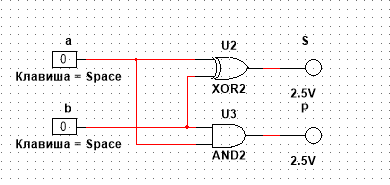
\includegraphics[width=0.62\textwidth]{lab2_half.png}
\caption{Модель полусумматора в среде Multisim}
\label{fig:ha_ms}
\end{figure}

Проверка выполнена полным перебором четырёх входных наборов. Результаты приведены в таблице~\ref{tab:ha_res}.

\begin{table}[H]
\caption{Результаты моделирования полусумматора}
\label{tab:ha_res}
\centering\small
\begin{tabularx}{\textwidth}{|C|C|C|C|C|C|C|}
\hline
a ($X$) & b ($Y$) & $X + Y$ & Пробник S & Пробник p & $2P + S$ & Соответ\-ствие \\ \hline
0 & 0 & 0 & 0 & 0 & 0 & да \\ \hline
0 & 1 & 1 & 1 & 0 & 1 & да \\ \hline
1 & 0 & 1 & 1 & 0 & 1 & да \\ \hline
1 & 1 & 2 & 0 & 1 & 2 & да \\ \hline
\end{tabularx}
\end{table}

Двоичное число $P S$, образованное выходами, на всех наборах равно арифметической сумме входов, и результаты совпадают с таблицей~\ref{tab:ha}. Функционирование полусумматора подтверждено.

% ======================= 4 =======================
\section{Синтез одноразрядного комбинационного сумматора}

\subsection{Исходные данные}

Функционирование одноразрядного сумматора задано таблицей истинности (таблица~\ref{tab:fa}), где $X$, $Y$~--- разряды слагаемых, $Z$~--- перенос из младшего разряда, $S$~--- разряд суммы, $P$~--- перенос в старший разряд.

\begin{table}[H]
\caption{Таблица истинности одноразрядного сумматора}
\label{tab:fa}
\centering\small
\begin{tabularx}{0.85\textwidth}{|C|C|C|C|C|C|}
\hline
№ набора & $X$ & $Y$ & $Z$ & $S$ & $P$ \\ \hline
0 & 0 & 0 & 0 & 0 & 0 \\ \hline
1 & 0 & 0 & 1 & 1 & 0 \\ \hline
2 & 0 & 1 & 0 & 1 & 0 \\ \hline
3 & 0 & 1 & 1 & 0 & 1 \\ \hline
4 & 1 & 0 & 0 & 1 & 0 \\ \hline
5 & 1 & 0 & 1 & 0 & 1 \\ \hline
6 & 1 & 1 & 0 & 0 & 1 \\ \hline
7 & 1 & 1 & 1 & 1 & 1 \\ \hline
\end{tabularx}
\end{table}

\subsection{Аналитические выражения в СДНФ}

Функция $S$ равна единице на наборах 1, 2, 4, 7, функция $P$~--- на наборах 3, 5, 6, 7 (таблица~\ref{tab:fa}). Запись функций в СДНФ:
\begin{equation}
S = \inv{X}\,\inv{Y} Z \vee \inv{X} Y \inv{Z} \vee X \inv{Y}\,\inv{Z} \vee X Y Z,
\end{equation}
\begin{equation}
P = \inv{X} Y Z \vee X \inv{Y} Z \vee X Y \inv{Z} \vee X Y Z,
\end{equation}
\noindent где $X$, $Y$~--- разряды слагаемых;\\
$Z$~--- перенос из младшего разряда;\\
$S$~--- разряд суммы;\\
$P$~--- перенос в старший разряд.

\subsection{Минимизация}

Минимизация выполнена по картам Карно (рисунок~\ref{fig:kmap}). Строки карт соответствуют значениям $X$, столбцы~--- значениям $YZ$ в коде Грея.

\begin{figure}[H]
\centering
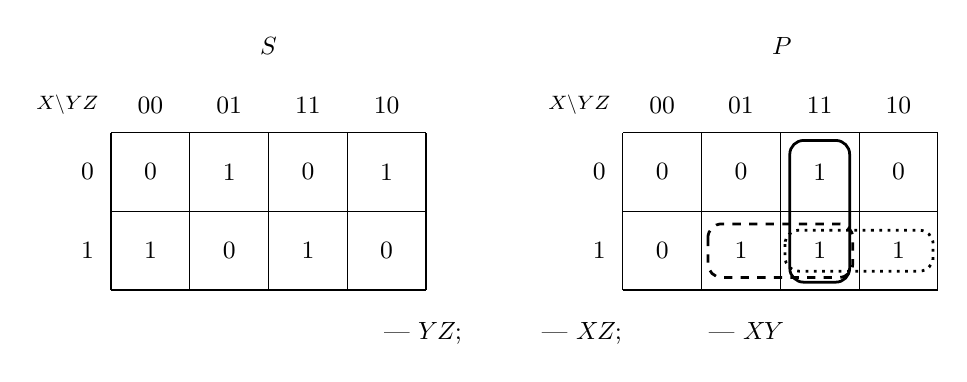
\begin{tikzpicture}[font=\small, x=1cm, y=1cm]
\foreach \xs/\name/\ra/\rb in {0/S/{0,1,0,1}/{1,0,1,0}, 6.5/P/{0,0,1,0}/{0,1,1,1}} {
 \begin{scope}[xshift=\xs cm]
  \node at (2,1.1) {$\name$};
  \foreach \c/\l in {0/00,1/01,2/11,3/10} \node at (\c+0.5,0.35) {\l};
  \node[anchor=east] at (-0.05,0.35) {\scriptsize $X \backslash YZ$};
  \node at (-0.3,-0.5) {0}; \node at (-0.3,-1.5) {1};
  \draw (0,0) grid (4,-2);
  \foreach \v [count=\c from 0] in \ra \node at (\c+0.5,-0.5) {\v};
  \foreach \v [count=\c from 0] in \rb \node at (\c+0.5,-1.5) {\v};
 \end{scope}}
\begin{scope}[xshift=6.5cm]
  \draw[rounded corners=5pt, line width=1pt] (2.12,-0.1) rectangle (2.88,-1.9);
  \draw[rounded corners=5pt, line width=1pt, dashed] (1.08,-1.16) rectangle (2.92,-1.84);
  \draw[rounded corners=5pt, line width=1pt, dotted] (2.06,-1.24) rectangle (3.94,-1.76);
\end{scope}
\node[font=\small] at (5.25,-2.55) {сплошной контур~--- $YZ$; штриховой~--- $XZ$; пунктирный~--- $XY$};
\end{tikzpicture}
\caption{Карты Карно функций суммы $S$ и переноса $P$}
\label{fig:kmap}
\end{figure}

На карте функции $S$ единицы расположены в шахматном порядке: ни одна пара единиц не находится в соседних клетках. Следовательно, склеивание невозможно, и СДНФ~(5) является минимальной ДНФ функции $S$. Функция $S$ равна единице при нечётном числе единиц среди аргументов, что соответствует сумме по модулю два:
\begin{equation}
S = X \oplus Y \oplus Z,
\end{equation}
\noindent где $X$, $Y$, $Z$~--- входы сумматора;\\
$S$~--- разряд суммы.

На карте функции $P$ единицы покрываются тремя контурами по две клетки. Каждый контур исключает одну переменную, что даёт минимальную ДНФ:
\begin{equation}
P = X Y \vee X Z \vee Y Z,
\end{equation}
\noindent где $X$, $Y$, $Z$~--- входы сумматора;\\
$P$~--- перенос в старший разряд.

Выражение~(8) преобразовано для совместного использования с выражением~(7) промежуточного сигнала $X \oplus Y$. Из СДНФ~(6) вынесением за скобки получено
\begin{equation}
P = X Y (Z \vee \inv{Z}) \vee Z (\inv{X} Y \vee X \inv{Y}) = X Y \vee Z \cdot (X \oplus Y),
\end{equation}
\noindent где $X$, $Y$, $Z$~--- входы сумматора;\\
$P$~--- перенос в старший разряд.

\subsection{Выбор варианта реализации}

Сравнение вариантов реализации сумматора по сложности приведено в таблице~\ref{tab:fa_cost}. Сложность оценена по Квайну~--- суммарным числом входов логических элементов.

\begin{table}[H]
\caption{Сравнение вариантов реализации одноразрядного сумматора}
\label{tab:fa_cost}
\centering\small
\begin{tabularx}{\textwidth}{|L|L|c|}
\hline
\multicolumn{1}{|c|}{Вариант} & \multicolumn{1}{c|}{Состав элементов} & Цена по Квайну \\ \hline
СДНФ~(5) для $S$ и минимальная ДНФ~(8) для $P$ в базисе И, ИЛИ, НЕ & 3 НЕ, 4 И3, 1 ИЛИ4 (для $S$); 3 И2, 1 ИЛИ3 (для $P$) & 28 \\ \hline
Выражения~(7) и~(9) с элементами «Исключающее ИЛИ» & 2 XOR2, 2 И2, 1 ИЛИ2 & 10 \\ \hline
\end{tabularx}
\end{table}

Для реализации выбран второй вариант. Он требует в 2,8 раза меньше входов элементов, а сигнал $X \oplus Y$ используется одновременно для формирования суммы~(7) и переноса~(9). Схема этого варианта состоит из двух полусумматоров (DD1, DD2 и DD3, DD4) и элемента ИЛИ (DD5), объединяющего их переносы. Схема электрическая принципиальная приведена на рисунке~\ref{fig:fa}.

\begin{figure}[H]
\centering
\begin{tikzpicture}[line width=0.5pt, font=\small, scale=1.2, every node/.style={transform shape}]
\node[left] at (0,0.9) {$Z$};
\node[left] at (0,-0.4) {$X$};
\node[left] at (0,-1.2) {$Y$};
% DD1 XOR(X,Y)
\draw (2.2,-1.5) rectangle (3.2,-0.1); \node at (2.7,-0.35) {=1};
\draw (0,-0.4) -- (2.2,-0.4); \draw (0,-1.2) -- (2.2,-1.2);
\fill (1.2,-0.4) circle (1.6pt); \fill (1.6,-1.2) circle (1.6pt);
% DD2 AND(X,Y)
\draw (2.2,-3.3) rectangle (3.2,-2.1); \node at (2.7,-2.35) {\&};
\draw (1.2,-0.4) -- (1.2,-2.4) -- (2.2,-2.4);
\draw (1.6,-1.2) -- (1.6,-3.0) -- (2.2,-3.0);
% DD3 XOR(Z, t)
\draw (4.6,0.1) rectangle (5.6,1.5); \node at (5.1,1.25) {=1};
\draw (0,0.9) -- (4.6,0.9);
\draw (3.2,-0.8) -- (3.9,-0.8); \fill (3.9,-0.8) circle (1.6pt);
\draw (3.9,-0.8) -- (3.9,0.4) -- (4.6,0.4);
\draw (5.6,0.8) -- (8.8,0.8) node[right] {$S$};
% DD4 AND(Z,t)
\draw (4.6,-1.9) rectangle (5.6,-0.7); \node at (5.1,-0.95) {\&};
\fill (4.2,0.9) circle (1.6pt);
\draw (4.2,0.9) -- (4.2,-1.1) -- (4.6,-1.1);
\draw (3.9,-0.8) -- (3.9,-1.6) -- (4.6,-1.6);
% DD5 OR
\draw (6.8,-2.6) rectangle (7.8,-1.2); \node at (7.3,-1.45) {1};
\draw (5.6,-1.3) -- (6.0,-1.3) -- (6.0,-1.6) -- (6.8,-1.6);
\draw (3.2,-2.7) -- (6.4,-2.7) -- (6.4,-2.2) -- (6.8,-2.2);
\draw (7.8,-1.9) -- (8.8,-1.9) node[right] {$P$};
\node[font=\scriptsize] at (2.7,0.1) {DD1};
\node[font=\scriptsize] at (2.7,-3.5) {DD2};
\node[font=\scriptsize] at (5.1,1.7) {DD3};
\node[font=\scriptsize] at (5.1,-2.1) {DD4};
\node[font=\scriptsize] at (7.3,-2.8) {DD5};
\node[font=\scriptsize, above] at (3.55,-0.8) {$X \oplus Y$};
\end{tikzpicture}
\caption{Схема электрическая принципиальная одноразрядного комбинационного сумматора}
\label{fig:fa}
\end{figure}

% ======================= 5 =======================
\section{Моделирование одноразрядного сумматора}

Модель сумматора введена в среде Multisim в соответствии со схемой на рисунке~\ref{fig:fa} и приведена на рисунке~\ref{fig:fa_ms}. Входы $X$, $Y$, $Z$ задаются интерактивными цифровыми константами a, b, P\_i; элементы U5 (XOR2) и U2 (AND2) образуют первый полусумматор, элементы U1 (XOR2) и U4 (AND2)~--- второй, элемент U3 (OR2) формирует перенос. Выходы $S$ и $P$ отображаются пробниками S и P\_i\_plus\_1.

\begin{figure}[H]
\centering
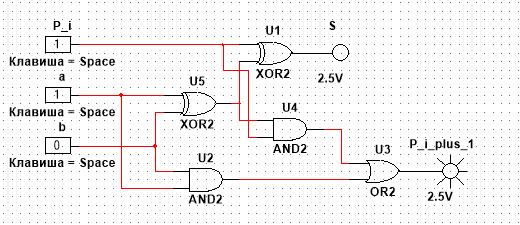
\includegraphics[width=0.8\textwidth]{lab2_full.png}
\caption{Модель одноразрядного сумматора в среде Multisim ($Z = 1$, $X = 1$, $Y = 0$)}
\label{fig:fa_ms}
\end{figure}

На рисунке~\ref{fig:fa_ms} зафиксирован набор $X = 1$, $Y = 0$, $Z = 1$: пробник S погашен, пробник P\_i\_plus\_1 светится, что соответствует сумме $1 + 0 + 1 = 10_2$. Результаты проверки на всех восьми наборах приведены в таблице~\ref{tab:fa_res}.

\begin{table}[H]
\caption{Результаты моделирования одноразрядного сумматора}
\label{tab:fa_res}
\centering\small
\begin{tabularx}{\textwidth}{|C|C|C|C|C|C|C|C|}
\hline
a ($X$) & b ($Y$) & P\_i ($Z$) & $X + Y + Z$ & Пробник S & \makecell{Пробник\\P\_i\_\\plus\_1} & $2P + S$ & Соответ\-ствие \\ \hline
0 & 0 & 0 & 0 & 0 & 0 & 0 & да \\ \hline
0 & 0 & 1 & 1 & 1 & 0 & 1 & да \\ \hline
0 & 1 & 0 & 1 & 1 & 0 & 1 & да \\ \hline
0 & 1 & 1 & 2 & 0 & 1 & 2 & да \\ \hline
1 & 0 & 0 & 1 & 1 & 0 & 1 & да \\ \hline
1 & 0 & 1 & 2 & 0 & 1 & 2 & да \\ \hline
1 & 1 & 0 & 2 & 0 & 1 & 2 & да \\ \hline
1 & 1 & 1 & 3 & 1 & 1 & 3 & да \\ \hline
\end{tabularx}
\end{table}

На всех наборах двоичное число $P S$ равно арифметической сумме трёх входов, результаты совпадают с таблицей~\ref{tab:fa}. Функционирование сумматора подтверждено.

% ======================= 6 =======================
\section{Исследование АЛУ К155ИП3 (SN74181)}

\subsection{Назначение и выводы микросхемы}

ИС К155ИП3 представляет собой четырёхразрядное АЛУ, выполняющее над операндами $A$ и $B$ шестнадцать логических и шестнадцать арифметических операций. Условное графическое обозначение микросхемы приведено на рисунке~\ref{fig:alu_ugo}.

\begin{figure}[H]
\centering
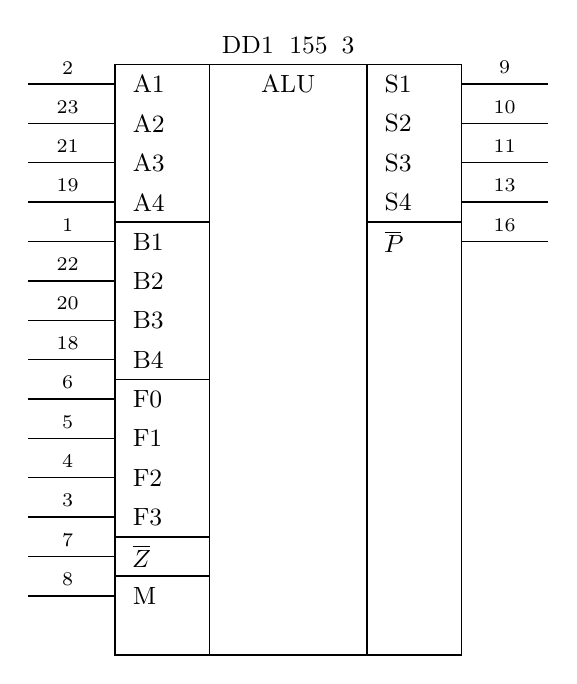
\begin{tikzpicture}[line width=0.5pt, font=\small, x=1cm, y=1cm]
\def\h{0.5}
\draw (0,0) rectangle (4.4,-15*\h);
\draw (1.2,0) -- (1.2,-15*\h);
\draw (3.2,0) -- (3.2,-15*\h);
\node at (2.2,-0.5*\h) {ALU};
\draw (0,-4*\h) -- (1.2,-4*\h);
\draw (0,-8*\h) -- (1.2,-8*\h);
\draw (0,-12*\h) -- (1.2,-12*\h);
\draw (0,-13*\h) -- (1.2,-13*\h);
\foreach \r/\lab/\pin/\iq in {0/A1/2/0,1/A2/23/0,2/A3/21/0,3/A4/19/0,4/B1/1/0,5/B2/22/0,6/B3/20/0,7/B4/18/0,8/F0/6/0,9/F1/5/0,10/F2/4/0,11/F3/3/0,12/$\overline{Z}$/7/0,13/M/8/0} {
  \node[anchor=west] at (0.1,{-(\r+0.5)*\h}) {\lab};
  \draw (-1.1,{-(\r+0.5)*\h}) -- (0,{-(\r+0.5)*\h});
  \node[above, font=\scriptsize] at (-0.6,{-(\r+0.5)*\h}) {\pin};
}
\draw (3.2,-4*\h) -- (4.4,-4*\h);
\foreach \r/\lab/\pin in {0/S1/9,1/S2/10,2/S3/11,3/S4/13,4/$\overline{P}$/16} {
  \node[anchor=west] at (3.3,{-(\r+0.5)*\h}) {\lab};
  \draw (4.4,{-(\r+0.5)*\h}) -- (5.5,{-(\r+0.5)*\h});
  \node[above, font=\scriptsize] at (4.95,{-(\r+0.5)*\h}) {\pin};
}
\node[above] at (2.2,0) {DD1 К155ИП3};
\end{tikzpicture}
\caption{Условное графическое обозначение ИС К155ИП3}
\label{fig:alu_ugo}
\end{figure}

Назначение выводов, их обозначения в модели 74181N среды Multisim и подключение к органам управления и индикации схемы исследования приведены в таблице~\ref{tab:alu_pins}. В модели 74181N выводы поименованы по технической документации SN74181 для интерпретации с активным низким уровнем данных; в работе используется эквивалентная интерпретация с активным высоким уровнем данных, принятая в методических указаниях~[1]. В этой интерпретации вход переноса $\overline{Z}$ и выход переноса $\overline{P}$ имеют активный низкий уровень.

\begin{table}[H]
\caption{Назначение выводов ИС К155ИП3 и их подключение}
\label{tab:alu_pins}
\centering\small
\begin{tabularx}{\textwidth}{|c|c|c|c|L|}
\hline
\makecell{Обозначение\\по [1]} & \makecell{Номер\\вывода} & \makecell{Имя вывода\\в 74181N} & \makecell{Элемент\\схемы} & \multicolumn{1}{c|}{Назначение} \\ \hline
A1--A4 & 2, 23, 21, 19 & \textasciitilde A0--\textasciitilde A3 & SA10--SA7 & Операнд $A$ (A1~--- младший разряд) \\ \hline
B1--B4 & 1, 22, 20, 18 & \textasciitilde B0--\textasciitilde B3 & SA6--SA3 & Операнд $B$ (B1~--- младший разряд) \\ \hline
F0--F3 & 6, 5, 4, 3 & S0--S3 & F0--F3 & Код выполняемой операции \\ \hline
$\overline{Z}$ & 7 & CN & SA2 & Вход переноса (активный уровень 0) \\ \hline
M & 8 & M & SA1 & Режим: 0~--- арифметический, 1~--- логический \\ \hline
S1--S4 & 9, 10, 11, 13 & \textasciitilde F0--\textasciitilde F3 & HLA1--HLA4 & Результат (S1~--- младший разряд) \\ \hline
$\overline{P}$ & 16 & CN4 & HLA5 & Выход переноса (активный уровень 0) \\ \hline
--- & 14, 15, 17 & AEQB, \textasciitilde P, \textasciitilde G & --- & Выход сравнения и выходы ускоренного переноса; не используются~[1] \\ \hline
\end{tabularx}
\end{table}

\subsection{Функции, выполняемые микросхемой}

Операции, используемые в работе, и их коды приведены в таблицах~\ref{tab:alu_arith} и~\ref{tab:alu_logic} по данным~[1]. Знак X обозначает безразличное значение.

\begin{table}[H]
\caption{Арифметические операции ИС К155ИП3 ($M = 0$)}
\label{tab:alu_arith}
\centering\small
\begin{tabularx}{\textwidth}{|C|C|C|C|C|C|}
\hline
$\overline{Z}$ & F3 & F2 & F1 & F0 & Операция \\ \hline
0 & 0 & 0 & 0 & 0 & $A + 1$ \\ \hline
1 & 0 & 0 & 0 & 0 & $A$ \\ \hline
0 & 0 & 0 & 1 & 1 & 0000 \\ \hline
1 & 0 & 0 & 1 & 1 & 1111 \\ \hline
0 & 0 & 1 & 1 & 0 & $A - B$ \\ \hline
1 & 0 & 1 & 1 & 0 & $A - B - 1$ \\ \hline
0 & 1 & 0 & 0 & 1 & $A + B + 1$ \\ \hline
1 & 1 & 0 & 0 & 1 & $A + B$ \\ \hline
0 & 1 & 1 & 0 & 0 & $A + A + 1$ \\ \hline
1 & 1 & 1 & 0 & 0 & $A + A$ \\ \hline
0 & 1 & 1 & 1 & 1 & $A$ \\ \hline
1 & 1 & 1 & 1 & 1 & $A - 1$ \\ \hline
\end{tabularx}
\end{table}

\begin{table}[H]
\caption{Логические операции ИС К155ИП3 ($M = 1$)}
\label{tab:alu_logic}
\centering\small
\begin{tabularx}{\textwidth}{|c|c|c|c|C||c|c|c|c|C|}
\hline
F3 & F2 & F1 & F0 & Операция & F3 & F2 & F1 & F0 & Операция \\ \hline
0 & 0 & 0 & 0 & $\inv{A}$ & 1 & 0 & 0 & 0 & $\inv{A} \vee B$ \\ \hline
0 & 0 & 0 & 1 & $\inv{A \vee B}$ & 1 & 0 & 0 & 1 & $\inv{A \oplus B}$ \\ \hline
0 & 0 & 1 & 0 & $\inv{A}\,B$ & 1 & 0 & 1 & 0 & $B$ \\ \hline
0 & 0 & 1 & 1 & 0 & 1 & 0 & 1 & 1 & $A B$ \\ \hline
0 & 1 & 0 & 0 & $\inv{A B}$ & 1 & 1 & 0 & 0 & 1 \\ \hline
0 & 1 & 0 & 1 & $\inv{B}$ & 1 & 1 & 0 & 1 & $A \vee \inv{B}$ \\ \hline
0 & 1 & 1 & 0 & $A \oplus B$ & 1 & 1 & 1 & 0 & $A \vee B$ \\ \hline
0 & 1 & 1 & 1 & $A\,\inv{B}$ & 1 & 1 & 1 & 1 & $A$ \\ \hline
\end{tabularx}
\end{table}

В арифметическом режиме микросхема выполняет двоичное сложение четырёхразрядных слагаемых, одно из которых определяется кодом F0--F3, с учётом входного переноса. Для операции сложения
\begin{equation}
A + B + c_0 = S + 2^4 \cdot c_4, \qquad c_0 = \inv{\overline{Z}}, \quad c_4 = \inv{\overline{P}},
\end{equation}
\noindent где $A$, $B$~--- значения операндов, вычисляемые по формуле~(1);\\
$S$~--- значение результата на выходах S1--S4;\\
$c_0$~--- входной перенос, $\overline{Z}$~--- уровень на входе переноса;\\
$c_4$~--- выходной перенос, $\overline{P}$~--- уровень на выходе переноса.

Вычитание выполняется сложением уменьшаемого с дополнительным кодом вычитаемого. Инверсный код четырёхразрядного числа $\inv{B}$ равен $2^4 - 1 - B$, поэтому при $c_0 = 1$
\begin{equation}
A + \inv{B} + 1 = A - B + 2^4,
\end{equation}
\noindent где $A$~--- уменьшаемое;\\
$B$~--- вычитаемое;\\
$\inv{B}$~--- поразрядная инверсия вычитаемого.

Из формулы~(11) следует, что при $A \geq B$ результат $S = A - B$ сопровождается выходным переносом $c_4 = 1$ ($\overline{P} = 0$), а при $A < B$ результат представлен в дополнительном коде и $c_4 = 0$ ($\overline{P} = 1$, заём).

\subsection{Схема исследования}

Схема исследования собрана в среде Multisim по образцу методических указаний~[1, рис.~4] и приведена на рисунке~\ref{fig:alu_ms}. Уровни на входах задаются интерактивными цифровыми константами: SA10--SA7~--- операнд $A$, SA6--SA3~--- операнд $B$, SA2~--- вход переноса $\overline{Z}$, SA1~--- режим M, F0--F3~--- код операции. Результат S1--S4 и выходной перенос $\overline{P}$ отображаются логическими пробниками HLA1--HLA5 с порогом срабатывания 2,5~В.

Для проверки собранной схемы все входы установлены в ноль. Этому состоянию по таблице~\ref{tab:alu_arith} соответствует операция $A + 1$ при $A = 0000$. Ожидаемый результат $S = 0001$ без переноса: светятся пробники HLA1 (S1~=~1) и HLA5 ($\overline{P} = 1$), что и зафиксировано на рисунке~\ref{fig:alu_ms}.

\begin{figure}[H]
\centering
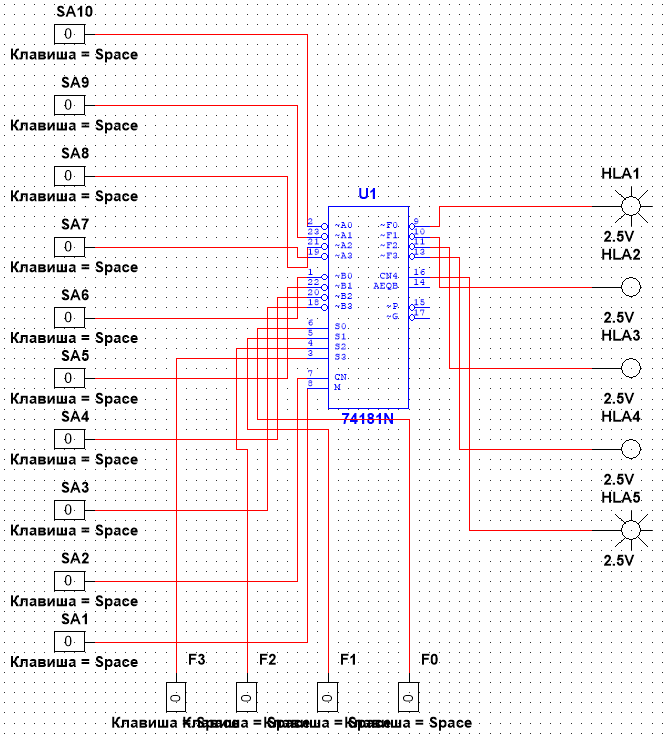
\includegraphics[width=0.6\textwidth]{lab2_alu_a1.png}
\caption{Схема исследования ИС К155ИП3 в среде Multisim (все входы равны 0, операция $A + 1$)}
\label{fig:alu_ms}
\end{figure}

\subsection{Исследование логических операций}

В логическом режиме ($M = 1$, SA1~=~1) исследованы три операции над заданными операндами: поразрядная конъюнкция, поразрядная дизъюнкция и сумма по модулю два. Состояния схемы приведены на рисунках~\ref{fig:and}--\ref{fig:xor}, результаты~--- в таблице~\ref{tab:logic_res}. Значения операндов и результата записаны от старшего разряда к младшему (A4\ldots A1, B4\ldots B1, S4\ldots S1).

\begin{figure}[H]
\centering
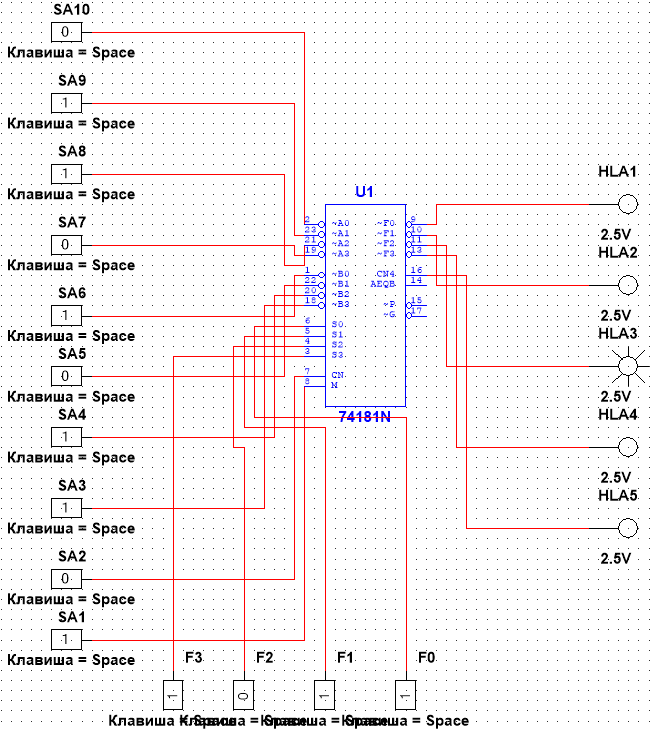
\includegraphics[width=0.52\textwidth]{lab2_and.png}
\caption{Поразрядная конъюнкция $A B$: $A = 0110$, $B = 1101$, код операции 1011}
\label{fig:and}
\end{figure}

\begin{figure}[H]
\centering
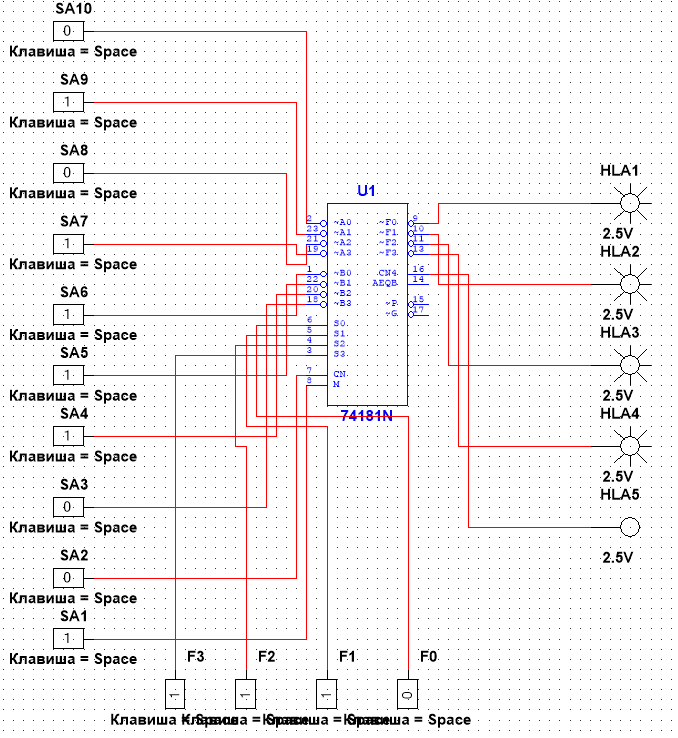
\includegraphics[width=0.52\textwidth]{lab2_or.png}
\caption{Поразрядная дизъюнкция $A \vee B$: $A = 1010$, $B = 0111$, код операции 1110}
\label{fig:or}
\end{figure}

\begin{figure}[H]
\centering
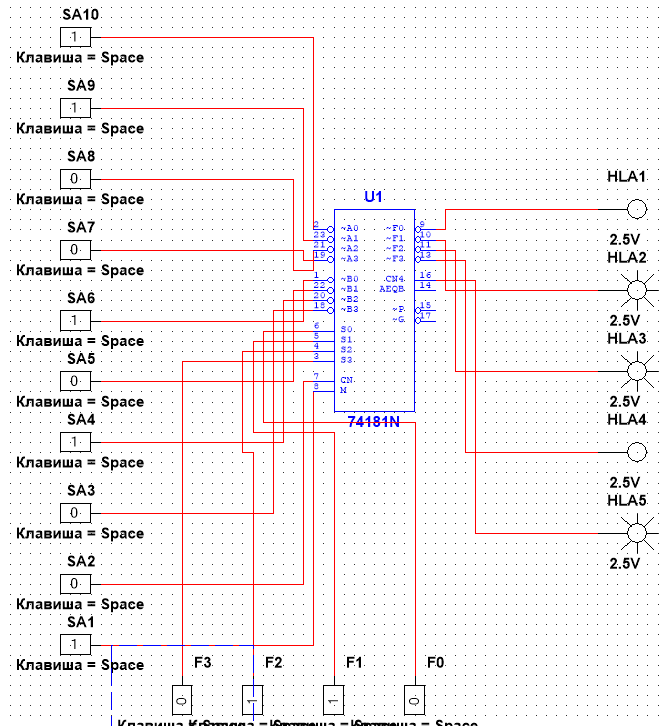
\includegraphics[width=0.52\textwidth]{lab2_xor.png}
\caption{Сумма по модулю два $A \oplus B$: $A = 0011$, $B = 0101$, код операции 0110}
\label{fig:xor}
\end{figure}

\begin{table}[H]
\caption{Результаты исследования логических операций ($M = 1$)}
\label{tab:logic_res}
\centering\small
\begin{tabularx}{\textwidth}{|C|c|c|c|c|C|C|}
\hline
Операция & \makecell{Код\\F3\ldots F0} & $A$ & $B$ & \makecell{Ожидаемый\\результат} & \makecell{Светящиеся\\пробники} & \makecell{Результат\\S4\ldots S1} \\ \hline
$A B$ & 1011 & 0110 & 1101 & 0100 & HLA3 & 0100 \\ \hline
$A \vee B$ & 1110 & 1010 & 0111 & 1111 & HLA1--HLA4 & 1111 \\ \hline
$A \oplus B$ & 0110 & 0011 & 0101 & 0110 & HLA2, HLA3 & 0110 \\ \hline
\end{tabularx}
\end{table}

Во всех трёх случаях результат совпадает с ожидаемым. Каждый разряд результата определяется только одноимёнными разрядами операндов, что подтверждает поразрядный характер логических операций. Уровень на входе переноса SA2 на результат логических операций не влияет. Выход переноса $\overline{P}$ в логическом режиме не несёт информации о результате: его состояние определяется внутренними сигналами генерации и распространения переноса (при операции $A \oplus B$ пробник HLA5 светится, при операциях $A B$ и $A \vee B$ погашен) и при анализе не учитывается.

\subsection{Исследование арифметических операций}

В арифметическом режиме ($M = 0$, SA1~=~0) исследованы операции сложения и вычитания. Состояния схемы приведены на рисунках~\ref{fig:add} и~\ref{fig:sub}, результаты~--- в таблице~\ref{tab:arith_res}.

Для сложения $A + B$ по таблице~\ref{tab:alu_arith} установлен код 1001 и $\overline{Z} = 1$ (входной перенос отсутствует). Для вычитания $A - B$ установлен код 0110 и $\overline{Z} = 0$: входной перенос $c_0 = 1$ обеспечивает прибавление единицы при переходе от инверсного кода вычитаемого к дополнительному в соответствии с формулой~(11).

\begin{figure}[H]
\centering
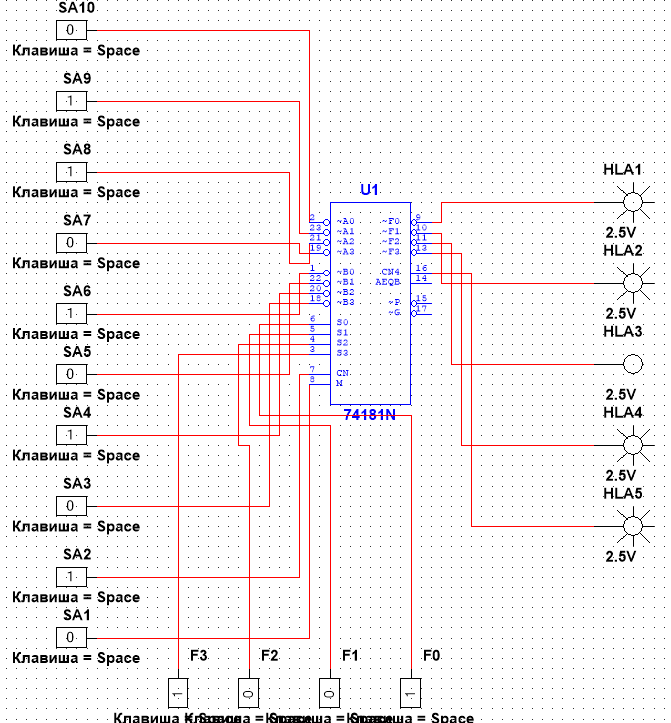
\includegraphics[width=0.52\textwidth]{lab2_add.png}
\caption{Сложение $A + B$: $A = 0110$, $B = 0101$, код операции 1001, $\overline{Z} = 1$}
\label{fig:add}
\end{figure}

\begin{figure}[H]
\centering
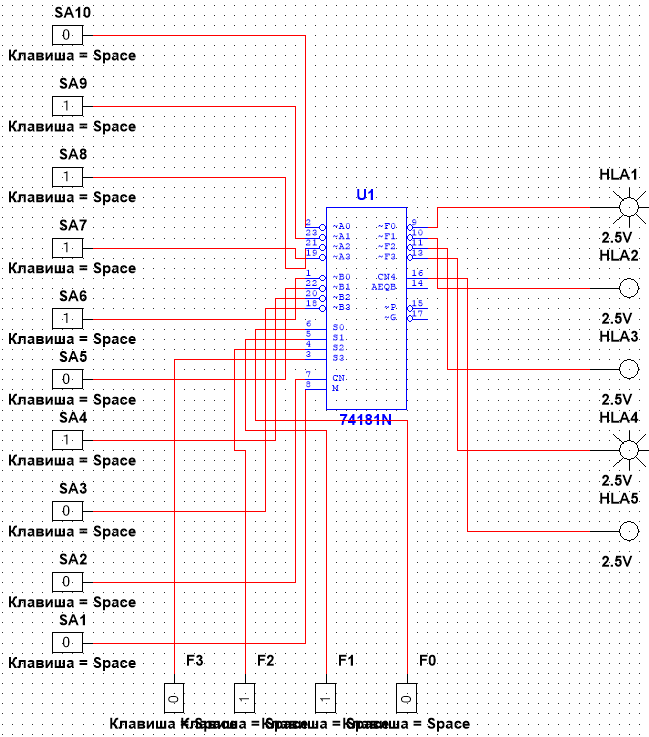
\includegraphics[width=0.52\textwidth]{lab2_sub.png}
\caption{Вычитание $A - B$: $A = 1110$, $B = 0101$, код операции 0110, $\overline{Z} = 0$}
\label{fig:sub}
\end{figure}

\begin{table}[H]
\caption{Результаты исследования арифметических операций ($M = 0$)}
\label{tab:arith_res}
\centering\small
\begin{tabularx}{\textwidth}{|C|c|c|c|c|C|C|C|}
\hline
Операция & \makecell{Код\\F3\ldots F0} & $\overline{Z}$ & $A$ & $B$ & \makecell{Светящиеся\\пробники} & \makecell{Результат\\S4\ldots S1} & $\overline{P}$ \\ \hline
$A + B$ & 1001 & 1 & \makecell{0110\\(6)} & \makecell{0101\\(5)} & HLA1, HLA2, HLA4, HLA5 & \makecell{1011\\(11)} & 1 \\ \hline
$A - B$ & 0110 & 0 & \makecell{1110\\(14)} & \makecell{0101\\(5)} & HLA1, HLA4 & \makecell{1001\\(9)} & 0 \\ \hline
\end{tabularx}
\end{table}

Анализ результатов по формулам~(10) и~(11):
\begin{gostlist}
\item сложение: $6 + 5 + 0 = 11 < 2^4$, следовательно, $S = 1011_2$ и $c_4 = 0$; пробник HLA5 светится ($\overline{P} = 1$), что подтверждает отсутствие переполнения;
\item вычитание: $\inv{B} = 1010_2$, $1110_2 + 1010_2 + 1 = 11001_2 = 25 = 9 + 2^4$, следовательно, $S = 1001_2 = 9$ и $c_4 = 1$; пробник HLA5 погашен ($\overline{P} = 0$), что соответствует $A \geq B$ (заём отсутствует).
\end{gostlist}

Результаты обеих операций совпадают с расчётными. Установлено, что вычитание в АЛУ выполняется без отдельного вычитающего узла~--- сложением уменьшаемого с дополнительным кодом вычитаемого, а выходной перенос при вычитании имеет смысл признака отсутствия заёма.

% ======================= ЗАКЛЮЧЕНИЕ =======================
\structsection{ЗАКЛЮЧЕНИЕ}

В ходе выполнения лабораторной работы получены следующие результаты.

1. Синтезирован полусумматор: $S = X \oplus Y$, $P = X Y$. Рассмотрены две модификации схемы: на элементах «Исключающее ИЛИ» и И (цена по Квайну 4) и в базисе И, ИЛИ, НЕ с совместным использованием сигнала $XY$ (цена 7). Моделирование модификации 1 на всех четырёх наборах подтвердило соответствие таблице истинности.

2. Синтезирован одноразрядный комбинационный сумматор. Установлено, что функция суммы $S = X \oplus Y \oplus Z$ не минимизируется в базисе И, ИЛИ, НЕ, а функция переноса минимизируется до $P = XY \vee XZ \vee YZ$. Выбрана реализация $P = XY \vee Z(X \oplus Y)$ из двух полусумматоров и элемента ИЛИ с ценой 10 против 28 для реализации в базисе И, ИЛИ, НЕ. Моделирование на всех восьми наборах подтвердило правильность синтеза.

3. Изучено АЛУ К155ИП3: режим работы задаётся входом M, операция~--- четырёхразрядным кодом F0--F3, вход и выход переноса в интерпретации с активным высоким уровнем данных имеют активный низкий уровень.

4. Исследованы логические операции $A B$, $A \vee B$, $A \oplus B$ на заданных операндах; результаты 0100, 1111, 0110 совпали с расчётными и подтвердили поразрядный характер логических операций.

5. Исследованы арифметические операции: $0110 + 0101 = 1011$ без выходного переноса и $1110 - 0101 = 1001$ с выходным переносом $c_4 = 1$. Подтверждено, что вычитание выполняется сложением с дополнительным кодом вычитаемого при входном переносе $c_0 = 1$.

% ======================= ИСТОЧНИКИ =======================
\structsection{СПИСОК ИСПОЛЬЗОВАННЫХ ИСТОЧНИКОВ}

\begin{enumerate}[label=\arabic*, leftmargin=*, labelindent=\parindent, itemsep=0pt, align=left]
\item Вербова, Н.\,М. Изучение элементов и узлов ЭВМ : сборник описаний лабораторных работ по курсу «Архитектура ЭВМ» / Н.\,М.~Вербова.~--- Санкт-Петербург : СПбГПУ, 2011.~--- 58~с.
\end{enumerate}

\end{document}
